\documentclass[conference]{IEEEtran}
\IEEEoverridecommandlockouts
% The preceding line is only needed to identify funding in the first footnote. If that is unneeded, please comment it out.
\usepackage{cite}
\usepackage{amsmath,amssymb,amsfonts}
\usepackage{algorithmic}
\usepackage{graphicx}
\usepackage{textcomp}
\usepackage{romannum}
\usepackage{enumitem}   


\def\BibTeX{{\rm B\kern-.05em{\sc i\kern-.025em b}\kern-.08em
    T\kern-.1667em\lower.7ex\hbox{E}\kern-.125emX}}
\begin{document}

\title{CS6290: Reading Summary \Romannum{2}}

\author{\IEEEauthorblockN{Yang Ji}
\IEEEauthorblockA{ID:\ 56064832 \\
yangji@comp.hkbu.edu.hk \\
Dept.\ of Computer Science}
}

\maketitle

\section{Summary of Paper \cite{castro1999practical}}


\subsection{Problem Statement}
This paper aims to develop a new replication algorithm to solve Byzantine fault problem efficiently.
%
In particular, it mainly focuses on the asynchronous environment and tries to reduce the response time by adopting many optimizations. 
%
Therefore, how to efficiently improve the system performance without satisfying any security still remained a huge challenge in that era.

\subsection{Problem Significance}
In the distributed system, there is no centralized parties to store and manage node information which can monitor the network running.
%
And some network nodes might perform a wide variety of Byzantine behaviors like message delay, corruption, crashes and so on.
%
Hence, it is of significance for a peer-to-peer network to reach a final consensus in an efficient manner.
 
\subsection{Preliminaries}
\subsubsection{Replication} 
Replication can be used to improve the performance and fault tolerance in the distributed system.
%
It has two basic modes: passive and active.
%
(\romannum{1}) Passive replication (also called primary-backup or master-slave replication) adopts an operating mode in which the primary server is responsible for receiving requests from clients and transmits these requests to the back-ups. 
%
(\romannum{2}) Active replication (also called state machine replication, SMR) ensures that all synchronized servers execute the same set of operations in the same order.

In the traditional Byzantine fault tolerance problem, SMR is applied to ensure the correctness of the whole system due to the failure check of message integrity.
%
Afterwards, introduced public-key cryptography makes BFT with passive replication real.

\subsubsection{Message Authentication Code (MAC)}
In cryptography, message authentication code (MAC) is used to ensure the massage's data integrity and authenticity.
%
In particular, it consists of three main algorithms:

\begin{enumerate}[label=(\roman*)]
    \item \textbf{Key-Generator.} Given a security parameter $1^{\lambda}$, it outputs a key $k$.
    \item \textbf{Signing.} Using the key $k$, it can output a tag $x$ according to the message $m$.
    \item \textbf{Verifying.} Given a tuple $(k, m, Signing(k, x))$, it outputs a decision bit (0 or 1) to tell whether the message m is authentic.
\end{enumerate}

\subsection{State of the Art}
At that time, some protocols implemented in the system SecureRing and Rampart were mainly based on the strong assumption of the synchrony network.
%
The safety could be compromised when there exists malicious attacks from some corrupted nodes.
%
What's more, the cryptographic overhead of public-key scheme could be seen as the major latency in Rampart. 

\begin{figure}[ht]
    \centering
    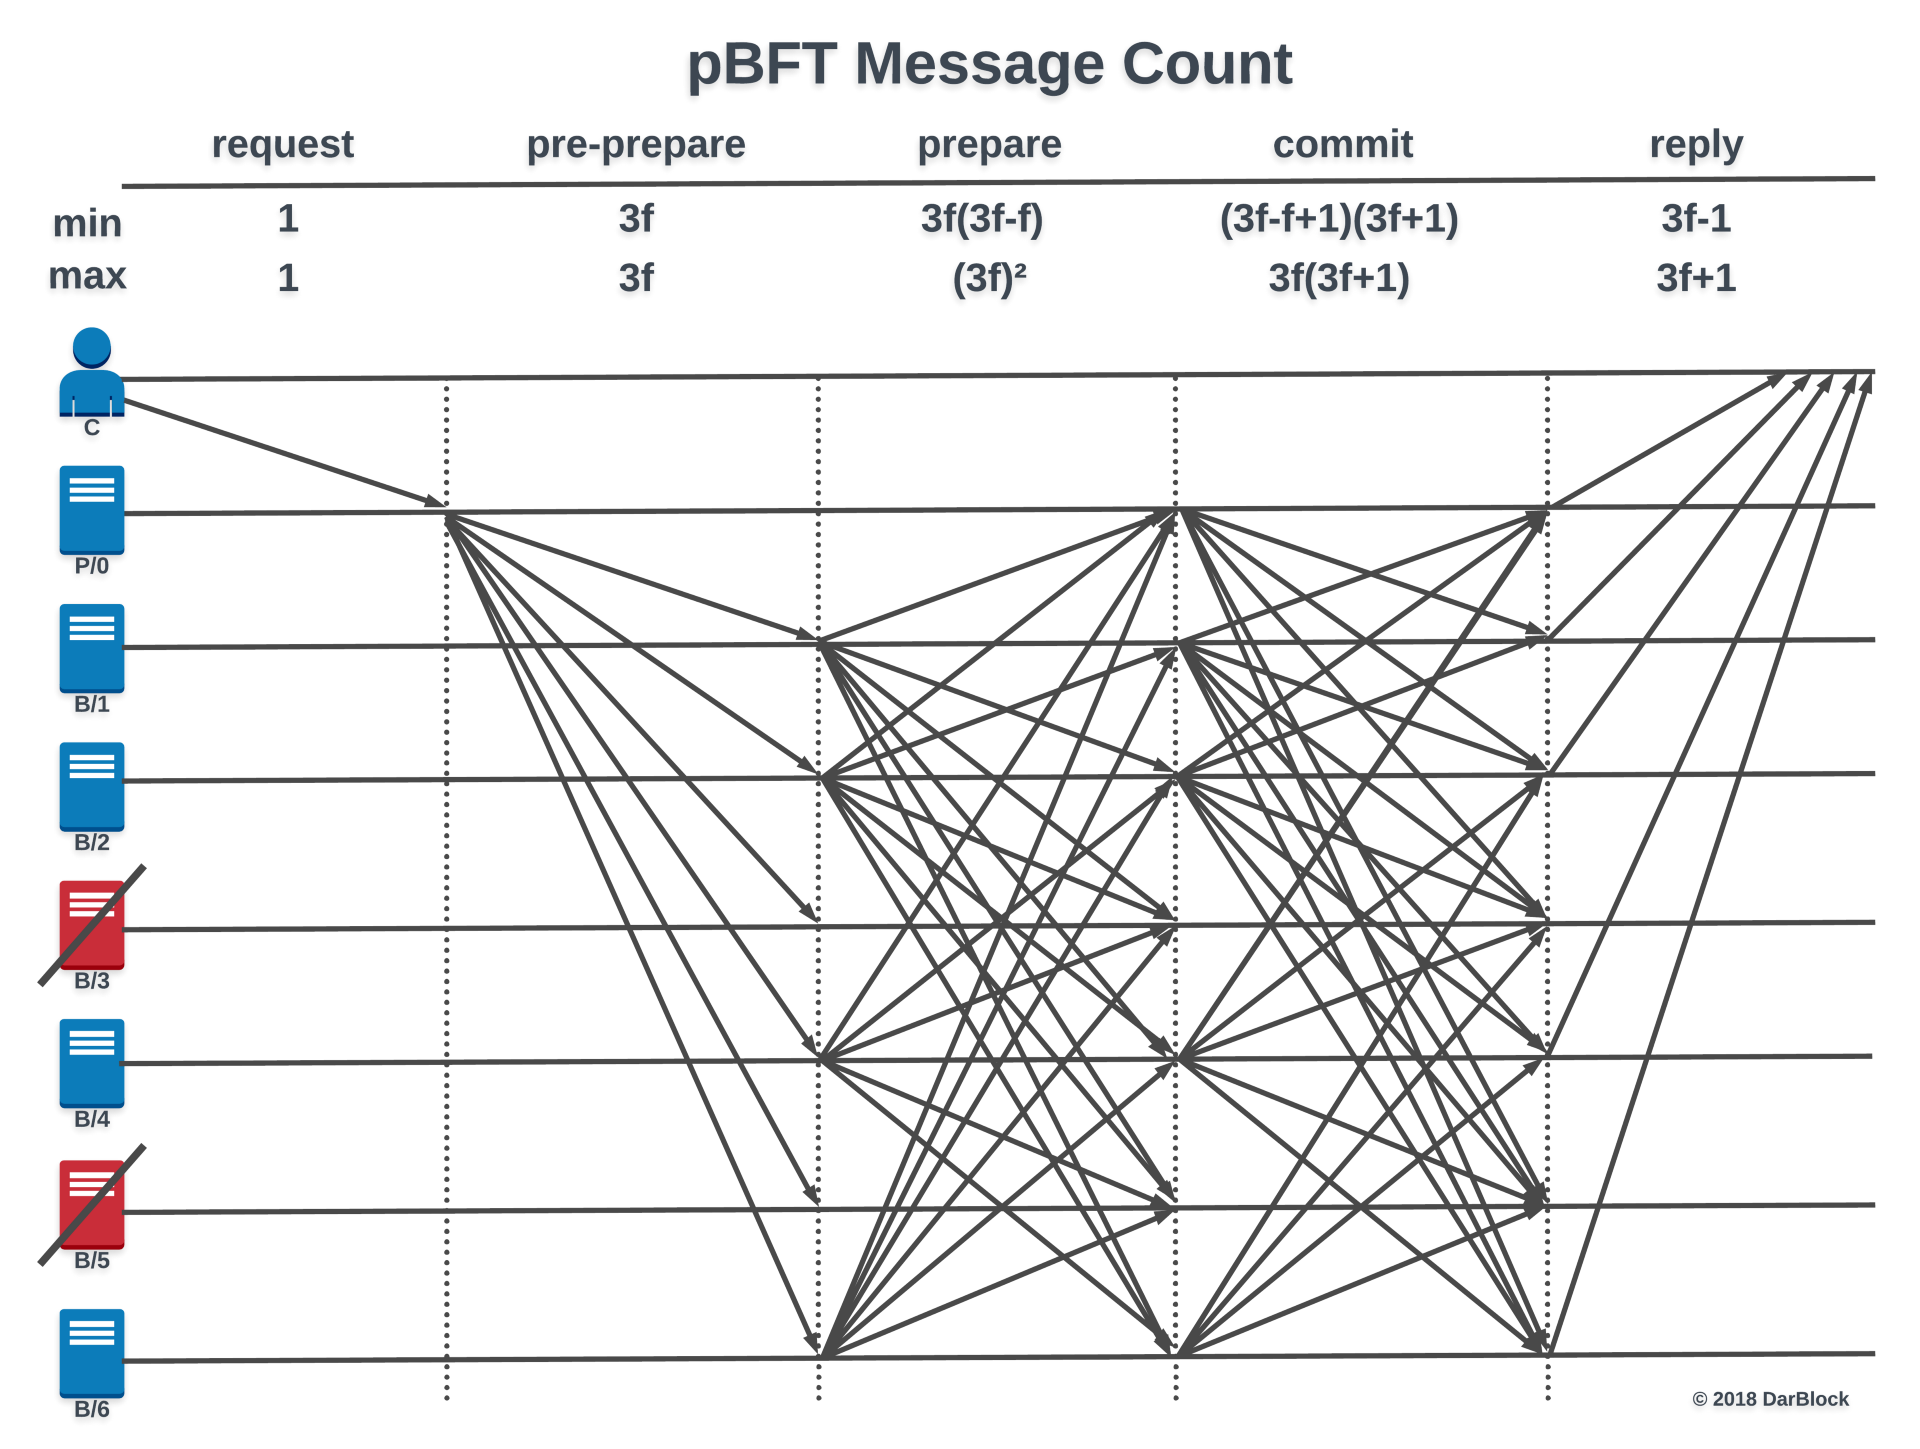
\includegraphics[width= 0.95\linewidth]{fig/PBFT.png}
    \caption{Normal Case Operations}
    \label{pbft}
\end{figure}

\subsection{Contributions}
The goals of three phase protocols are two-fold.
%
One is to establish the total order of execution of requests in the pre-prepare and prepare phase.
%
The other one is to ensure that requests are ordered consistently across views (configurations of replicas with a primary $p = v\ mod\ {\mid} N \mid$) by the commit operations.

\subsection{Remaining Questions}
Guidelines: Here you should try to discuss any remaining questions to be solved or any possible future directions based on the result of the paper.

\section{Summary of Paper \cite{CurtmolaGKO06}}

\subsection{Problem Statement}
Guidelines: Here you should explicitly summarize the problem targeted by the paper. A rough and brief example might be as follows.
%
The paper targets the problem of searching encrypted outsourced data on the cloud.
%
Particularly, how to enable a client to perform search and get the correct search result when both the cloud database and query keywords are encrypted?

\subsection{Problem Significance}
Guidelines: Here you should explain why the problem targeted by the paper is important and has value.
%
In particular, what is the motivation of this paper?


\subsection{State of the Art}

Guidelines: Here you should describe the state of the art as reflected in the paper at that time.
%



\subsection{Contributions}
Guidelines: Here you should summarize the contributions of the paper in your own words.
%
For example, you may evaluate the contributions from the following perspectives: novelty of problem formulation, novelty of the technical solution, depth of theoretical analysis of the technical solution, positiveness of experimental evaluation result, etc.

\subsection{Remaining Questions}
Guidelines: Here you should try to discuss any remaining questions to be solved or any possible future directions based on the result of the paper.

\bibliographystyle{IEEEtran}
\bibliography{references}


\end{document}
